\documentclass[11pt]{article}
    \usepackage[english]{babel}
    \usepackage[top=1.25cm, left=2.5cm, bottom =1.25cm, right =2.5cm]{geometry}
    \usepackage[block=ragged, style=authoryear,sorting=ynt]{biblatex}
    \usepackage[nottoc,notlot,notlof]{tocbibind}
    \usepackage[longtable]{multirow}
    \usepackage[section]{placeins}
    \usepackage[titles]{tocloft}
    \usepackage{csquotes}
    \usepackage{fontspec}
    \usepackage{titlesec}
    \usepackage{float}
    \usepackage{setspace}
    \usepackage{longtable}
    \usepackage{array}
    \usepackage{rotating}
    \usepackage{colortbl}
    \usepackage{pgfgantt}
    \usepackage{xcolor}
    \usepackage{xparse}
    \usepackage{graphicx}
    \usepackage{lscape}
    \usepackage{parskip}
    \setmainfont{Arial}
    \onehalfspacing
    \setlength\parindent{0pt}
    \setlength{\parindent}{0em}
    \addbibresource{References.bib}
    \titleformat{\chapter}[hang] 
    {\normalfont\LARGE\bfseries}{\chaptertitlename\ \thechapter:}{0.5em}{} 
    \titlespacing*{\chapter}{0pt}{0pt}{1em}
    \setcounter{tocdepth}{3}% Include \subsubsection
    \setcounter{secnumdepth}{3}% Number \subsubsection
\begin{document}
\begin{titlepage}
    \centering
    {\LARGE\bfseries IN3046: Cloud Computing }

    \vspace{0.5cm}

    {\Large Coursework - Specification of Application}

    
\includegraphics[width=7.5cm, height=10cm]{Images/CUL Logo}

    \vspace{0.1cm}

    {\Large 04/03/2021}
    \vspace{0.5cm}

    {\large Dr . Maria Krotsiani}
    \vspace {0.5cm}

    \vspace*{\fill}

    {School of Mathematics, Computer Science and Engineering \\ City, University of London \\ London, UK \\ January 2021}
\end{titlepage}
\section{Requirements of Application}
We are proposing to build a command-line program to manage a user's passwords similarly to GNU/PASS \parencite{GNU/PASS}. The project dictates that it must be a cloud-based application. To adhere to this requirement we will be using Google Cloud \parencite{GoogleCloud} to host the server with MongoDB \parencite{MongoDB} as our database application. Users of the application will be able to manage their passwords and associated usernames for different accounts by generating and storing passwords which will be more difficult for an attacker to crack compared to a normal password. The user will have an account which is associated to their keychain. They can then log in to this to access their stored credentials. They will then be able to retrieve existing credentials as well as generate new ones via a set of commands. For example, if a user wanted to set up an account for Facebook, they would call 'register Facebook <USERNAME>' and a secure password will be generated and displayed to the user. Otherwise, if a password is entered, e.g. 'register Facebook <USERNAME> <PASSWORD>' it will add the account to their keychain instead.
\section{Typical Users}
The intended users are those individuals who are concerned with the management of their passwords. This is often the case as people have had to start using more complex passwords to protect their accounts from attackers. As the number of accounts a user has grows, so does the amount of passwords (providing they use unique password for each service). This means that the average person will have to remember a large number of complex passwords which don't have any meaning to them. Increasing the chances of them forgetting one. A password manager makes that much easier by putting them all in one place. This means the user only has to remember one complex passphrase. The password manager would have to be very secure for a user to trust their most important details with it. That is why this password manager can be deployed by users on their own servers, giving them finer control of access to their data. The users will be able to access their keychain from any device with an internet connection that can run Python (the client).
\section{Implementation}
The application will be coded using Python. The implementation will use symmetric encryption for transferring passwords so the server will be unable to see the passwords. The encryption key will be stored locally on the client alongside a username and password when you initially log in or register. Google cloud will be used to host the server, upon log in the password is hashed with the salt and compared to the one present in the database. If they match, the request is completed and the server will fetch the credentials from the database. Registration is similar but nothing is returned. Atlas, a management server for MongoDB will be used to monitor the status of the database and for testing. The PyMongo library will be used to integrate MongoDB into Python and web sockets will be used for data transmission between the server and client. We will be using Google Cloud which has integrations with MongoDB Atlas.
\section{Architecture of Application}
\begin{figure}
\centering
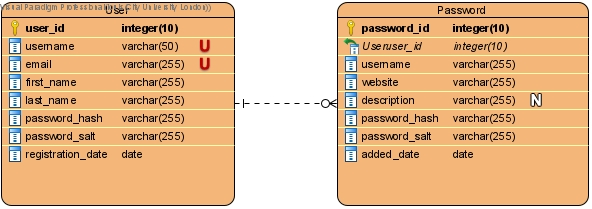
\includegraphics[width=1.0\textwidth]{diagrams/erd.jpg}
\caption{Entity Relationship Diagram}
\end{figure}
\begin{figure}
\centering
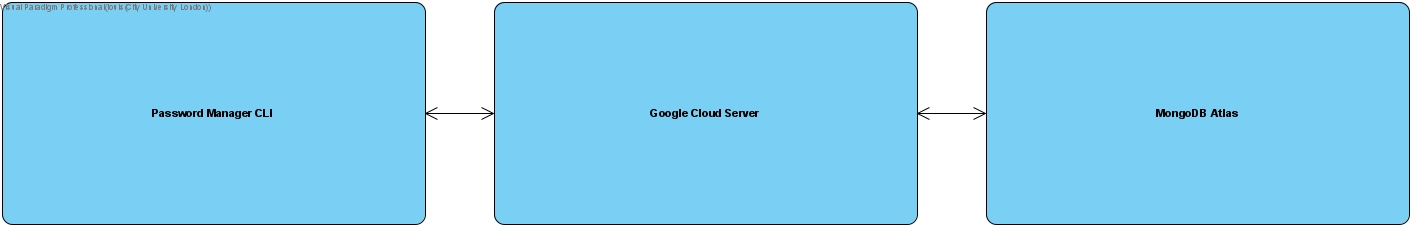
\includegraphics[width=1.0\textwidth]{diagrams/dd.jpg}
\caption{Deployment Diagram}
\end{figure}

\section{Distribution of Work}
To ensure that the work is evenly distributed between the team, we have divided the tasks as follows. All members will be taking part in every stage but each member will be in charge of a part of the project.
\par
L - Project Management, Deployment Diagram, Demo Video, Specification
\par
M - Google Cloud Authentication, MongoDB Integration, Presentation
\par
S - ERD, Presentation, Google Cloud SQL and Storage, Testing, Specification
\printbibliography[heading=bibintoc]
\end{document}